\documentclass[11pt,a4paper]{article}

\usepackage[T1]{fontenc}
\usepackage[margin=1in]{geometry}
\usepackage{amsmath}
\usepackage{amssymb}
\usepackage{array}
\usepackage{booktabs}
\usepackage{longtable}
\usepackage{float}
\usepackage{graphicx}
\usepackage{xcolor}
\usepackage{tikz}
\usetikzlibrary{arrows.meta,positioning,shapes.geometric,calc,fit}

\title{ELEC5803 HLS Exam Study\\Step-by-Step Solution to Question 1}
\author{}
\date{}

\tikzset{
  >={Latex[length=2mm]},
  block/.style={draw, rounded corners, align=center, minimum width=2.4cm, minimum height=0.9cm},
  smallblock/.style={draw, rounded corners, align=center, minimum width=1.8cm, minimum height=0.8cm},
  decision/.style={diamond, draw, aspect=2.0, align=center, inner sep=1pt, minimum width=2.6cm},
  startstop/.style={ellipse, draw, align=center, minimum width=2.4cm, minimum height=0.9cm},
  reg/.style={draw, rounded corners, fill=blue!6, align=center, minimum width=1.8cm, minimum height=0.9cm},
  fu/.style={draw, rounded corners, fill=green!7, align=center, minimum width=2.2cm, minimum height=1cm},
  ctrl/.style={draw, rounded corners, fill=orange!10, align=center, minimum width=2.5cm, minimum height=1cm},
  pred/.style={diamond, draw, aspect=1.8, align=center, inner sep=1.5pt, fill=yellow!10},
  dashedctrl/.style={dashed, -Latex},
  dfgop/.style={draw, circle, fill=blue!10, minimum size=8mm, inner sep=0pt, align=center},
  dfgio/.style={draw, rectangle, rounded corners, minimum width=1.2cm, minimum height=0.7cm, align=center},
  csbox/.style={draw, rounded corners, minimum width=5.2cm, minimum height=1.2cm},
  stg/.style={draw, rectangle, rounded corners, minimum width=2.1cm, minimum height=0.8cm, align=center},
}

\begin{document}
\maketitle

\section*{Course-slide basis}
This solution follows the same HLS flow used in the course slides:
\begin{itemize}
  \item \textbf{Slides 5:} \emph{Behavioral HDL to CDFG Translation or Compilation}, \emph{ASAP and ALAP Scheduling and Mobility}, and resource-constrained scheduling in \texttt{Slides/ELEC5803\_Slides5\_HLS Algorithms\_Part1.pdf}.
  \item \textbf{Slides 6:} scheduling versus binding/allocation, datapath synthesis, and compatibility-based sharing in \texttt{Slides/ELEC5803\_Slides6\_HLS Algorithms\_Part2.pdf}.
  \item \textbf{Slides 7:} FSM/FSMD-style controller realization in \texttt{Slides/ELEC5803\_Slides7\_Control Unit Design\_AA1.pdf}.
\end{itemize}

\section*{Important interpretation note}
The printed VHDL in the sample exam is clearly intended to implement \textbf{Stein's algorithm} (binary GCD), but it is not fully self-consistent as written:
\begin{itemize}
  \item the port declaration is syntactically incomplete,
  \item the ``both-even'' case of Stein's algorithm is missing,
  \item \texttt{shift\_count} is declared but never incremented,
  \item the final result should be restored by a left shift, i.e.\ multiplying by $2^{k}$.
\end{itemize}
Therefore, the solution below uses the \textbf{intended binary-GCD algorithm}, which is the only interpretation consistent with the comments in the code and with the exam questions on flowchart, DFG, scheduling, and hardware design.

\section*{1. Intended algorithm}
Let $k$ denote the number of common factors of $2$ removed from both operands.

\begin{enumerate}
  \item Load $x \leftarrow X\_IN$, $y \leftarrow Y\_IN$, $k \leftarrow 0$.
  \item If $x=0$, output $y$. If $y=0$, output $x$.
  \item Repeat until $x=y$:
  \begin{itemize}
    \item If $x$ and $y$ are both even, set $x \leftarrow x/2$, $y \leftarrow y/2$, $k \leftarrow k+1$.
    \item Else if $x$ is even, set $x \leftarrow x/2$.
    \item Else if $y$ is even, set $y \leftarrow y/2$.
    \item Else if $x>y$, set $x \leftarrow (x-y)/2$.
    \item Else set $y \leftarrow (y-x)/2$.
  \end{itemize}
  \item When $x=y$, output $\mathrm{GCD}=x \ll k$.
\end{enumerate}

\section*{2. Flowchart of the algorithm}
\begin{figure}[h!]
\centering
\resizebox{0.82\textwidth}{!}{%
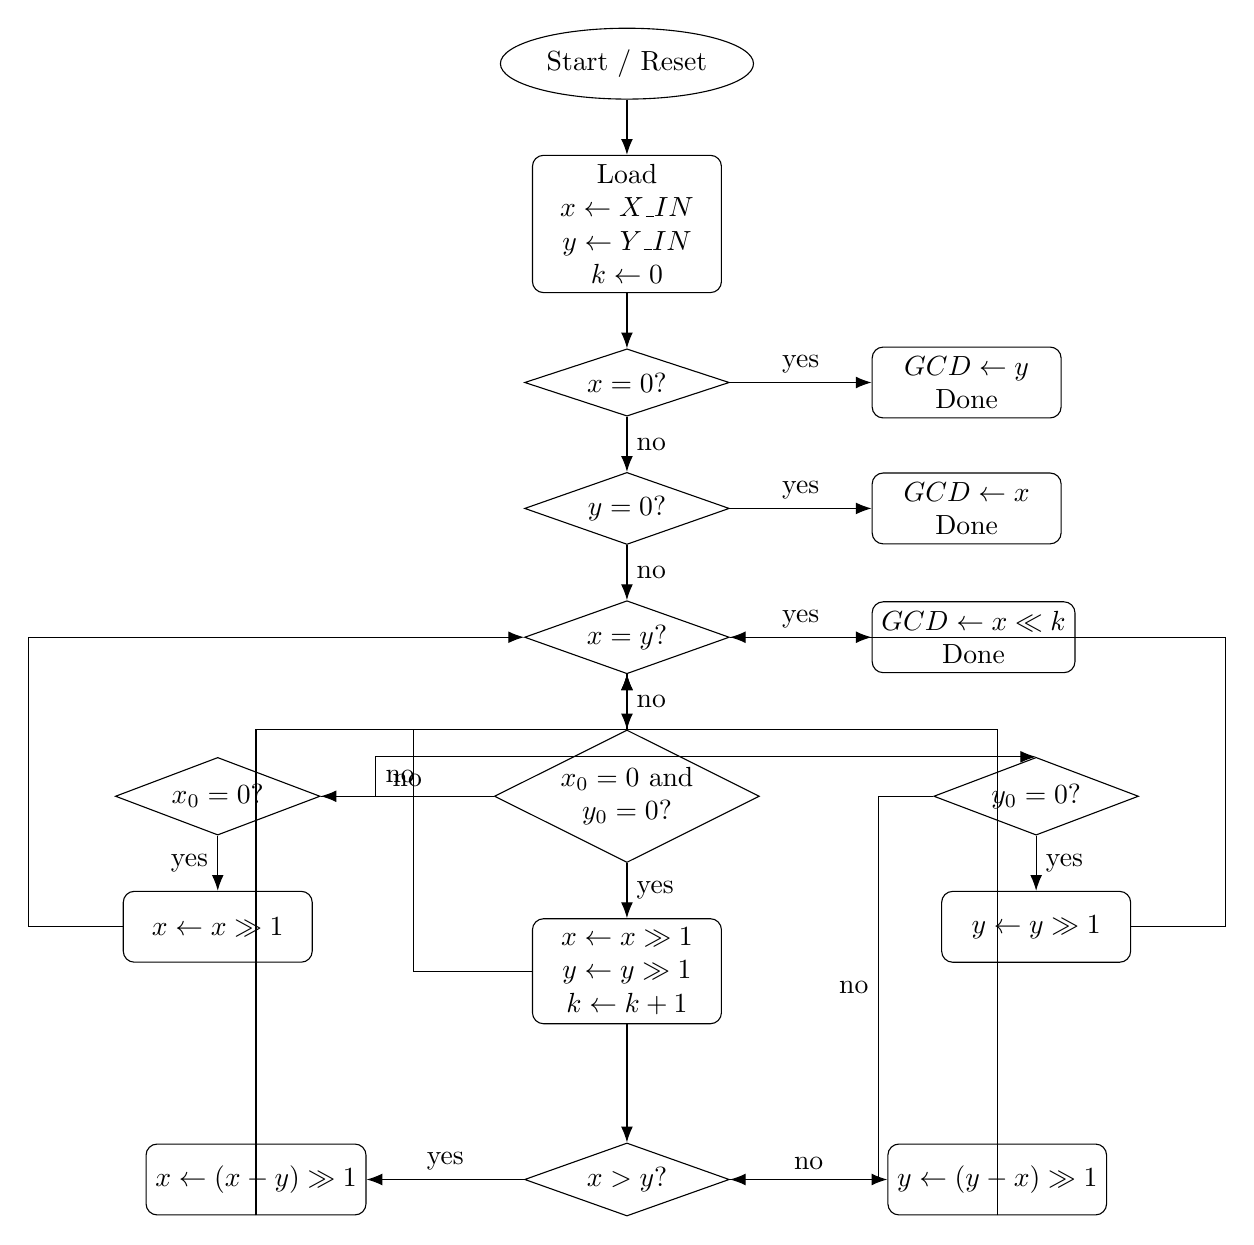
\begin{tikzpicture}[node distance=7mm and 9mm]
  \node[startstop] (start) {Start / Reset};
  \node[block, below=of start] (load) {Load\\$x\leftarrow X\_IN$\\$y\leftarrow Y\_IN$\\$k\leftarrow 0$};
  \node[decision, below=of load] (xzero) {$x=0$?};
  \node[block, right=18mm of xzero] (outy) {$GCD\leftarrow y$\\Done};
  \node[decision, below=of xzero] (yzero) {$y=0$?};
  \node[block, right=18mm of yzero] (outx) {$GCD\leftarrow x$\\Done};
  \node[decision, below=of yzero] (equal) {$x=y$?};
  \node[block, right=18mm of equal] (finish) {$GCD\leftarrow x \ll k$\\Done};
  \node[decision, below=of equal] (botheven) {$x_0=0$ and\\$y_0=0$?};
  \node[block, below=of botheven] (bothupd) {$x\leftarrow x \gg 1$\\$y\leftarrow y \gg 1$\\$k\leftarrow k+1$};
  \node[decision, left=22mm of botheven] (xeven) {$x_0=0$?};
  \node[block, below=of xeven] (xupd) {$x\leftarrow x \gg 1$};
  \node[decision, right=22mm of botheven] (yeven) {$y_0=0$?};
  \node[block, below=of yeven] (yupd) {$y\leftarrow y \gg 1$};
  \node[decision, below=15mm of bothupd] (gt) {$x>y$?};
  \node[block, left=20mm of gt] (xsub) {$x\leftarrow (x-y)\gg 1$};
  \node[block, right=20mm of gt] (ysub) {$y\leftarrow (y-x)\gg 1$};

  \draw[->] (start) -- (load);
  \draw[->] (load) -- (xzero);
  \draw[->] (xzero) -- node[above] {yes} (outy);
  \draw[->] (xzero) -- node[right] {no} (yzero);
  \draw[->] (yzero) -- node[above] {yes} (outx);
  \draw[->] (yzero) -- node[right] {no} (equal);
  \draw[->] (equal) -- node[above] {yes} (finish);
  \draw[->] (equal) -- node[right] {no} (botheven);
  \draw[->] (botheven) -- node[right] {yes} (bothupd);
  \draw[->] (botheven) -- node[above] {no} (xeven);
  \draw[->] (xeven) -- node[left] {yes} (xupd);
  \draw[->] (xeven.east) -- ++(7mm,0) |- node[pos=0.25, right] {no} (yeven.north);
  \draw[->] (yeven) -- node[right] {yes} (yupd);
  \draw[->] (yeven.west) -- ++(-7mm,0) |- node[pos=0.25, left] {no} (gt.east);
  \draw[->] (bothupd) -- (gt);
  \draw[->] (gt) -- node[above] {yes} (xsub);
  \draw[->] (gt) -- node[above] {no} (ysub);

  \draw[->] (xupd.west) -- ++(-12mm,0) |- ($(equal.west)+(-9mm,0)$) |- (equal.west);
  \draw[->] (yupd.east) -- ++(12mm,0) |- ($(equal.east)+(9mm,0)$) |- (equal.east);
  \draw[->] (xsub.south) |- ($(equal.south)+(0,-7mm)$) -| (equal.south);
  \draw[->] (ysub.south) |- ($(equal.south)+(0,-7mm)$) -| (equal.south);
  \draw[->] (bothupd.west) -- ++(-15mm,0) |- ($(equal.south)+(0,-7mm)$) -| (equal.south);
\end{tikzpicture}%
}
\caption{Flowchart for the intended Stein/binary-GCD algorithm. This is the natural control-flow representation corresponding to the behavior-to-CDFG discussion in Slides 5.}
\end{figure}

\clearpage
\section*{3. Data-flow graph (DFG) / sequencing view}
To match the style used in the course slides, it is better to separate:
\begin{itemize}
  \item an \textbf{unscheduled sequencing DFG}, which only shows operations and precedence edges, and
  \item a \textbf{scheduled DFG}, which groups the same operations into control steps.
\end{itemize}

This is the same presentation logic used in the Slides-5 examples around the HAL DFG and the scheduled DFG.

For one non-terminal iteration, the main arithmetic candidates are:
\[
\begin{aligned}
v_1 &: s_x = x \gg 1 \\
v_2 &: s_y = y \gg 1 \\
v_3 &: k_1 = k + 1 \\
v_4 &: d_{xy} = x - y \\
v_5 &: d_{yx} = y - x \\
v_6 &: n_x = d_{xy} \gg 1 \\
v_7 &: n_y = d_{yx} \gg 1 \\
v_8 &: g = x \ll k
\end{aligned}
\]
with dependencies $v_4 \rightarrow v_6$ and $v_5 \rightarrow v_7$.

\begin{figure}[h!]
\centering
\resizebox{\textwidth}{!}{%
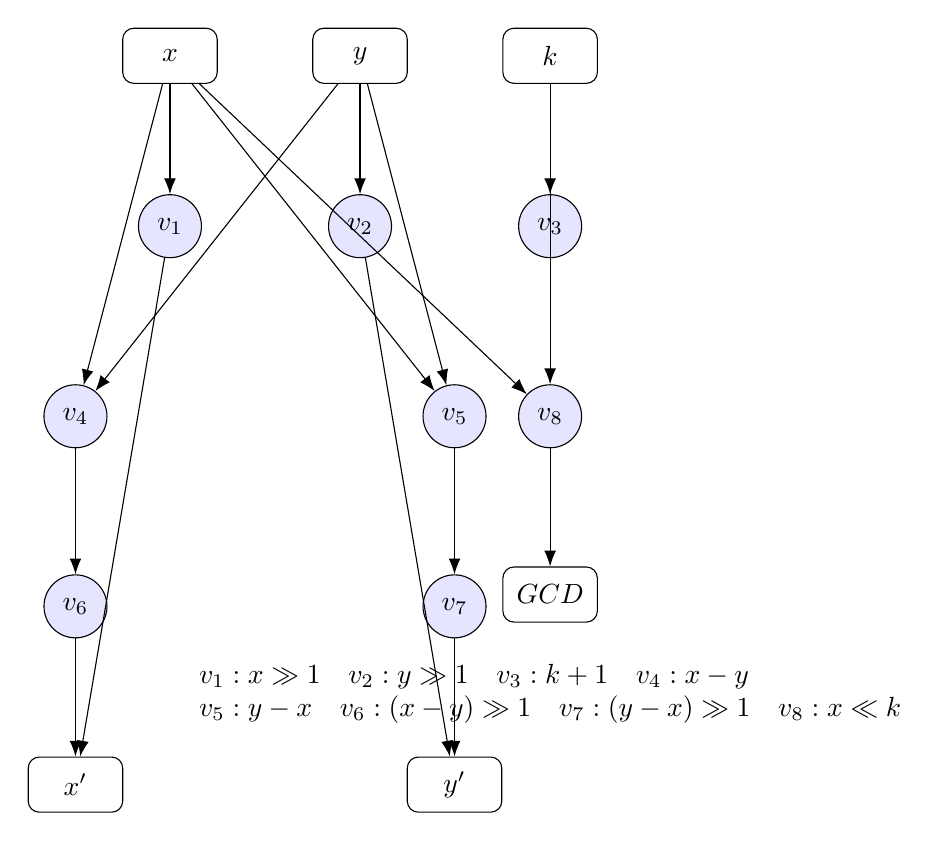
\begin{tikzpicture}[node distance=10mm and 12mm]
  \node[dfgio] (x) {$x$};
  \node[dfgio, right=12mm of x] (y) {$y$};
  \node[dfgio, right=12mm of y] (k) {$k$};

  \node[dfgop, below=14mm of x] (v1) {$v_1$};
  \node[dfgop, below=14mm of y] (v2) {$v_2$};
  \node[dfgop, below=14mm of k] (v3) {$v_3$};

  \node[dfgop, below=16mm of v1, xshift=-12mm] (v4) {$v_4$};
  \node[dfgop, below=16mm of v2, xshift=12mm] (v5) {$v_5$};

  \node[dfgop, below=16mm of v4] (v6) {$v_6$};
  \node[dfgop, below=16mm of v5] (v7) {$v_7$};
  \node[dfgop, below=16mm of v3] (v8) {$v_8$};

  \node[dfgio, below=15mm of v6] (xn) {$x'$};
  \node[dfgio, below=15mm of v7] (yn) {$y'$};
  \node[dfgio, below=15mm of v8] (gcd) {$GCD$};

  \draw[->] (x) -- (v1);
  \draw[->] (y) -- (v2);
  \draw[->] (k) -- (v3);
  \draw[->] (x) -- (v4);
  \draw[->] (y) -- (v4);
  \draw[->] (y) -- (v5);
  \draw[->] (x) -- (v5);
  \draw[->] (v4) -- (v6);
  \draw[->] (v5) -- (v7);
  \draw[->] (x) -- (v8);
  \draw[->] (k) -- (v8);
  \draw[->] (v1) -- (xn);
  \draw[->] (v6) -- (xn);
  \draw[->] (v2) -- (yn);
  \draw[->] (v7) -- (yn);
  \draw[->] (v8) -- (gcd);

  \node[below=4mm of gcd, align=left] {
    $v_1: x \gg 1$\quad
    $v_2: y \gg 1$\quad
    $v_3: k+1$\quad
    $v_4: x-y$\\
    $v_5: y-x$\quad
    $v_6: (x-y)\gg 1$\quad
    $v_7: (y-x)\gg 1$\quad
    $v_8: x \ll k$
  };
\end{tikzpicture}%
}
\caption{Unscheduled sequencing DFG for one Stein-algorithm iteration, drawn in the same operation-vertex style as the DFG figures in the course slides.}
\end{figure}

\begin{figure}[h!]
\centering
\resizebox{0.82\textwidth}{!}{%
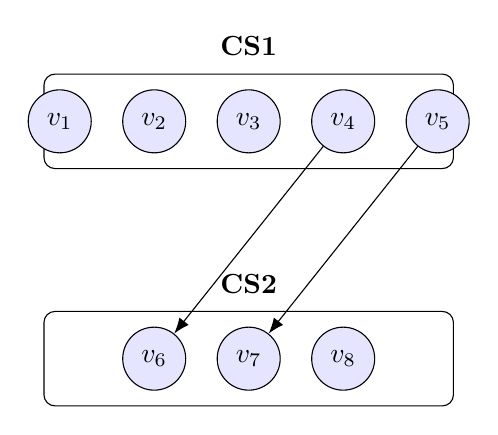
\begin{tikzpicture}[node distance=10mm and 10mm]
  \node[csbox] (cs1) {};
  \node[above=1mm of cs1] {\textbf{CS1}};
  \node[dfgop] (s1v1) at ($(cs1.center)+(-24mm,0)$) {$v_1$};
  \node[dfgop] (s1v2) at ($(cs1.center)+(-12mm,0)$) {$v_2$};
  \node[dfgop] (s1v3) at ($(cs1.center)+(0mm,0)$) {$v_3$};
  \node[dfgop] (s1v4) at ($(cs1.center)+(12mm,0)$) {$v_4$};
  \node[dfgop] (s1v5) at ($(cs1.center)+(24mm,0)$) {$v_5$};

  \node[csbox, below=18mm of cs1] (cs2) {};
  \node[above=1mm of cs2] {\textbf{CS2}};
  \node[dfgop] (s2v6) at ($(cs2.center)+(-12mm,0)$) {$v_6$};
  \node[dfgop] (s2v7) at ($(cs2.center)+(0mm,0)$) {$v_7$};
  \node[dfgop] (s2v8) at ($(cs2.center)+(12mm,0)$) {$v_8$};

  \draw[->] (s1v4) -- (s2v6);
  \draw[->] (s1v5) -- (s2v7);
\end{tikzpicture}%
}
\caption{Scheduled DFG in slide style: the same operation vertices grouped by control step. This corresponds to the ASAP schedule used in part (c).}
\end{figure}

\clearpage
\subsection*{3.1 Controller FSM for the minimum-area FSMD}
To match the control-unit style from Slides 7, the datapath can be driven by a Moore-style FSM whose states correspond to the main algorithm phases.

\begin{figure}[h!]
\centering
\resizebox{\textwidth}{!}{%
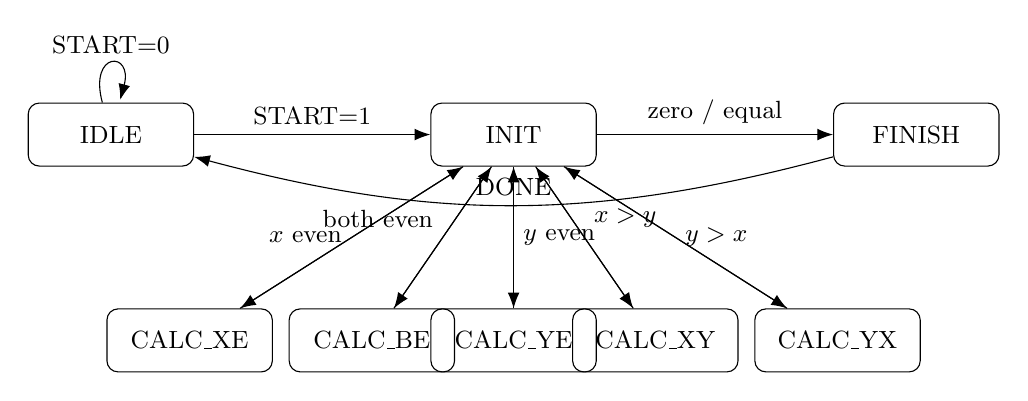
\begin{tikzpicture}[node distance=12mm and 16mm, font=\small]
  \node[stg] (idle) {IDLE};
  \node[stg, right=30mm of idle] (init) {INIT};
  \node[stg, right=30mm of init] (finish) {FINISH};

  \node[stg, below=18mm of idle, xshift=10mm] (xe) {CALC\_XE};
  \node[stg, below=18mm of init, xshift=-18mm] (be) {CALC\_BE};
  \node[stg, below=18mm of init] (ye) {CALC\_YE};
  \node[stg, below=18mm of init, xshift=18mm] (xy) {CALC\_XY};
  \node[stg, below=18mm of finish, xshift=-10mm] (yx) {CALC\_YX};

  \draw[->] (idle) edge[loop above] node {START=0} (idle);
  \draw[->] (idle) -- node[above] {START=1} (init);
  \draw[->] (init) -- node[above] {zero / equal} (finish);

  \draw[->] (init) -- node[above left] {both even} (be);
  \draw[->] (init) -- node[left] {$x$ even} (xe);
  \draw[->] (init) -- node[right] {$y$ even} (ye);
  \draw[->] (init) -- node[above right] {$x>y$} (xy);
  \draw[->] (init) -- node[right] {$y>x$} (yx);

  \draw[->] (be) -- (init);
  \draw[->] (xe) -- (init);
  \draw[->] (ye) -- (init);
  \draw[->] (xy) -- (init);
  \draw[->] (yx) -- (init);
  \draw[->] (finish) to[bend left=15] node[above] {DONE} (idle);
\end{tikzpicture}%
}
\caption{State-transition graph for the controller FSM. This is the same kind of FSM/STG representation used in the control-unit slides.}
\end{figure}

\begin{center}
\begin{tabular}{>{\raggedright\arraybackslash}p{1.7cm} >{\raggedright\arraybackslash}p{3.2cm} >{\raggedright\arraybackslash}p{3.0cm} >{\raggedright\arraybackslash}p{5.3cm}}
\toprule
Present state & Condition & Next state & Moore-state action / micro-operation \\
\midrule
IDLE & START=0 & IDLE & Wait; DONE=0 \\
IDLE & START=1 & INIT & Load $x\leftarrow X\_IN$, $y\leftarrow Y\_IN$, $k\leftarrow 0$ \\
INIT & $x=0$ & FINISH & $GCD \leftarrow y$ \\
INIT & $y=0$ & FINISH & $GCD \leftarrow x$ \\
INIT & $x=y$ & FINISH & $GCD \leftarrow x \ll k$ \\
INIT & $x_0=0 \land y_0=0$ & CALC\_BE & Select both-even path \\
INIT & $x_0=0 \land y_0=1$ & CALC\_XE & Select $x$-even path \\
INIT & $x_0=1 \land y_0=0$ & CALC\_YE & Select $y$-even path \\
INIT & $x_0=1 \land y_0=1 \land x>y$ & CALC\_XY & Select odd-odd, $x>y$ path \\
INIT & $x_0=1 \land y_0=1 \land y>x$ & CALC\_YX & Select odd-odd, $y>x$ path \\
CALC\_BE & unconditional & INIT & $x\leftarrow x\gg 1$, $y\leftarrow y\gg 1$, $k\leftarrow k+1$ \\
CALC\_XE & unconditional & INIT & $x\leftarrow x\gg 1$ \\
CALC\_YE & unconditional & INIT & $y\leftarrow y\gg 1$ \\
CALC\_XY & unconditional & INIT & $x\leftarrow (x-y)\gg 1$ \\
CALC\_YX & unconditional & INIT & $y\leftarrow (y-x)\gg 1$ \\
FINISH & unconditional & IDLE & DONE=1 \\
\bottomrule
\end{tabular}
\end{center}

\noindent
The table above plays the same role as the \emph{state transition table / direct structure table} in the FSM slides: it lists present state, transition condition, next state, and the state-associated actions.

\section*{4. ASAP and ALAP scheduling}
Slides 5 define:
\begin{itemize}
  \item \textbf{ASAP}: place each operation in the earliest possible control step.
  \item \textbf{ALAP}: place each operation in the latest possible control step without increasing the latency obtained from ASAP.
  \item \textbf{Mobility}: $\text{ALAP} - \text{ASAP}$.
\end{itemize}

Here we schedule the arithmetic DFG vertices $\{v_1,\ldots,v_8\}$ with the standard simplifying assumption used in scheduling exercises:
\begin{itemize}
  \item each arithmetic operation takes one control step,
  \item predicate evaluation belongs to the controller,
  \item unlimited resources are available for parts (c) ASAP/ALAP only.
\end{itemize}

\subsection*{4.1 Precedence constraints}
Only two true arithmetic dependencies exist inside the iteration kernel:
\[
v_4 \rightarrow v_6, \qquad v_5 \rightarrow v_7
\]
All of the other candidate results are produced directly from the current-state registers.

\subsection*{4.2 ASAP schedule}
The minimum achievable latency for this DFG is therefore \textbf{2 control steps}.

\begin{center}
\begin{tabular}{>{\raggedright\arraybackslash}p{2.3cm}cc}
\toprule
Operation & CS1 & CS2 \\
\midrule
$v_1: x \gg 1$ & $\bullet$ & \\
$v_2: y \gg 1$ & $\bullet$ & \\
$v_3: k+1$ & $\bullet$ & \\
$v_4: x-y$ & $\bullet$ & \\
$v_5: y-x$ & $\bullet$ & \\
$v_6: (x-y)\gg 1$ & & $\bullet$ \\
$v_7: (y-x)\gg 1$ & & $\bullet$ \\
$v_8: x \ll k$ & $\bullet$ & \\
\bottomrule
\end{tabular}
\end{center}

\subsection*{4.3 ALAP schedule}
Using the same total latency of 2 steps:

\begin{center}
\begin{tabular}{>{\raggedright\arraybackslash}p{2.3cm}cc}
\toprule
Operation & CS1 & CS2 \\
\midrule
$v_1: x \gg 1$ & & $\bullet$ \\
$v_2: y \gg 1$ & & $\bullet$ \\
$v_3: k+1$ & & $\bullet$ \\
$v_4: x-y$ & $\bullet$ & \\
$v_5: y-x$ & $\bullet$ & \\
$v_6: (x-y)\gg 1$ & & $\bullet$ \\
$v_7: (y-x)\gg 1$ & & $\bullet$ \\
$v_8: x \ll k$ & & $\bullet$ \\
\bottomrule
\end{tabular}
\end{center}

\subsection*{4.4 Mobility table}
\begin{center}
\begin{tabular}{cccc}
\toprule
Vertex & ASAP & ALAP & Mobility \\
\midrule
$v_1$ & 1 & 2 & 1 \\
$v_2$ & 1 & 2 & 1 \\
$v_3$ & 1 & 2 & 1 \\
$v_4$ & 1 & 1 & 0 \\
$v_5$ & 1 & 1 & 0 \\
$v_6$ & 2 & 2 & 0 \\
$v_7$ & 2 & 2 & 0 \\
$v_8$ & 1 & 2 & 1 \\
\bottomrule
\end{tabular}
\end{center}

\subsection*{4.5 Interpretation}
This result matches the course discussion in Slides 5:
\begin{itemize}
  \item subtraction nodes $v_4$ and $v_5$ have \textbf{zero mobility} because their shifted successors force them into control step 1,
  \item shifts on the current operands and the final restoration shift have \textbf{mobility 1},
  \item this mobility information is exactly what later guides hardware sharing and allocation.
\end{itemize}

\section*{5. Hardware design with minimum area}
For minimum area, the correct HLS strategy from Slides 6 is to \textbf{maximize hardware sharing} and allow a multi-cycle iterative implementation.

\subsection*{5.1 Datapath idea}
Use one shared arithmetic datapath:
\begin{itemize}
  \item registers: $R_x$, $R_y$, $R_k$, and an output register $R_g$,
  \item one shared ALU to perform subtraction and increment,
  \item one shared shifter to perform right shifts and the final left shift,
  \item one comparison/status block producing $x=0$, $y=0$, $x=y$, $x>y$, $x_0$, and $y_0$,
  \item multiplexers at ALU and shifter inputs,
  \item one FSM controller.
\end{itemize}

\begin{figure}[h!]
\centering
\resizebox{\textwidth}{!}{%
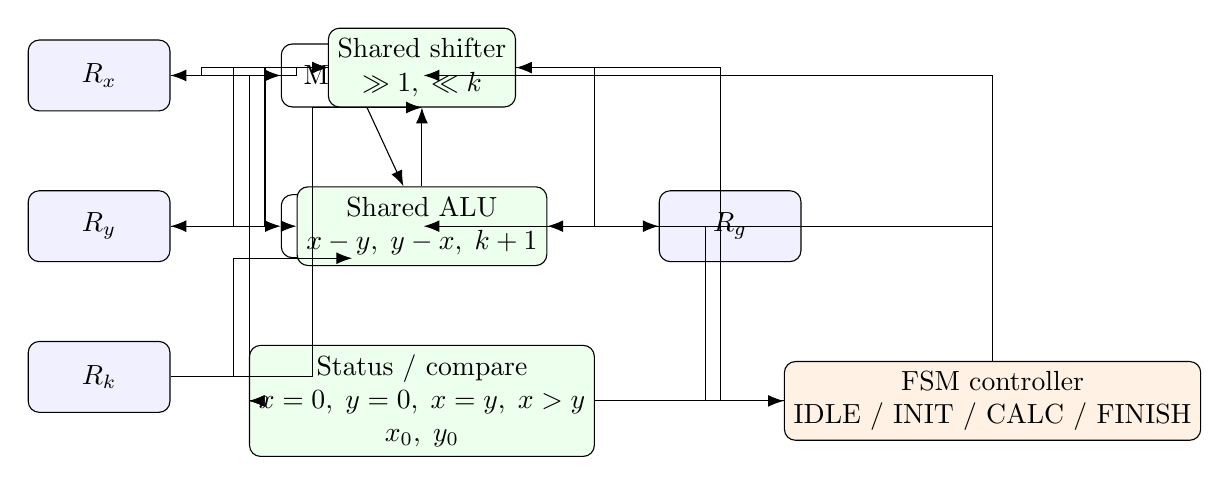
\begin{tikzpicture}[node distance=10mm and 10mm]
  \node[reg] (rx) {$R_x$};
  \node[reg, below=of rx] (ry) {$R_y$};
  \node[reg, below=of ry] (rk) {$R_k$};
  \node[reg, right=62mm of ry] (rg) {$R_g$};

  \node[smallblock, right=14mm of rx] (muxa) {MUX A};
  \node[smallblock, right=14mm of ry] (muxb) {MUX B};
  \node[fu, right=16mm of ry] (alu) {Shared ALU\\$x-y,\; y-x,\; k+1$};
  \node[fu, above=of alu] (shift) {Shared shifter\\$\gg 1,\; \ll k$};
  \node[fu, below=of alu] (cmp) {Status / compare\\$x=0,\; y=0,\; x=y,\; x>y$\\$x_0,\; y_0$};
  \node[ctrl, right=24mm of cmp] (fsm) {FSM controller\\IDLE / INIT / CALC / FINISH};

  \draw[->] (rx) -- (muxa);
  \draw[->] (ry) -- (muxb);
  \draw[->] (rk.east) -- ++(8mm,0) |- (muxb.south);
  \draw[->] (muxa) -- (alu);
  \draw[->] (muxb) -- (alu);
  \draw[->] (rx.east) -- ++(16mm,0) |- (shift.west);
  \draw[->] (ry.east) -- ++(12mm,0) |- (shift.west);
  \draw[->] (rk.east) -- ++(18mm,0) |- (shift.south);
  \draw[->] (alu) -- (shift);
  \draw[->] (shift.east) -- ++(10mm,0) |- (rg.west);
  \draw[->] (shift.west) -- ++(-16mm,0) |- (rx.east);
  \draw[->] (shift.west) -- ++(-12mm,0) |- (ry.east);
  \draw[->] (rx.east) -- ++(10mm,0) |- (cmp.west);
  \draw[->] (ry.east) -- ++(10mm,0) |- (cmp.west);
  \draw[->] (cmp) -- (fsm);
  \draw[->] (fsm.north) |- (muxa.east);
  \draw[->] (fsm.north) |- (muxb.east);
  \draw[->] (fsm.west) -- ++(-10mm,0) |- (alu.east);
  \draw[->] (fsm.west) -- ++(-8mm,0) |- (shift.east);
\end{tikzpicture}%
}
\caption{Minimum-area FSMD-style hardware. The same ALU and shifter are reused across multiple control steps, which is the key Slides-6 allocation idea for minimizing area.}
\end{figure}

\subsection*{5.2 Why this is minimum-area}
The hardware is area-efficient because:
\begin{itemize}
  \item only \textbf{one arithmetic unit} is used for all subtract and increment operations,
  \item only \textbf{one shifter} is used for all divide-by-2 and final restore operations,
  \item the algorithm is iterative, so throughput is sacrificed in exchange for hardware reuse,
  \item the controller sequences the shared datapath exactly as in the FSMD model from Slides 7.
\end{itemize}

\subsection*{5.3 Typical operation sequence}
One possible control realization is:
\begin{longtable}{p{2.3cm}p{10.5cm}}
\toprule
State & Action \\
\midrule
IDLE & Wait for \texttt{START=1}. \\
INIT & Load $R_x \leftarrow X\_IN$, $R_y \leftarrow Y\_IN$, $R_k \leftarrow 0$; check zero cases. \\
CALC\_BE & Both-even case: use shifter twice (or in two successive micro-operations) to update $x$ and $y$, then ALU for $k+1$. \\
CALC\_XE & $x$ even: shift $x$ right by one. \\
CALC\_YE & $y$ even: shift $y$ right by one. \\
CALC\_XY & Odd-odd and $x>y$: ALU computes $x-y$, then shifter computes $(x-y)\gg 1$, then write back to $R_x$. \\
CALC\_YX & Odd-odd and $y>x$: ALU computes $y-x$, then shifter computes $(y-x)\gg 1$, then write back to $R_y$. \\
FINISH & Use shifter for $x \ll k$, store to $R_g$, assert \texttt{DONE}. \\
\bottomrule
\end{longtable}

\noindent
This design uses the \textbf{fewest functional units}, but it needs the \textbf{largest number of control steps per iteration}.

\clearpage
\section*{6. Hardware design with minimum latency}
For minimum latency, the HLS goal changes: instead of maximizing reuse, we allocate more hardware so that as much work as possible is done in parallel during each loop iteration.

\subsection*{6.1 Datapath idea}
Compute all candidate next values in parallel:
\begin{itemize}
  \item one right shifter for $x \gg 1$,
  \item one right shifter for $y \gg 1$,
  \item one subtractor for $x-y$ followed by a shifter for $(x-y)\gg 1$,
  \item one subtractor for $y-x$ followed by a shifter for $(y-x)\gg 1$,
  \item one incrementer for $k+1$,
  \item one left shifter for the final $x \ll k$,
  \item parallel comparators for all branch conditions,
  \item multiplexers that select the correct next-state values.
\end{itemize}

\begin{figure}[h!]
\centering
\resizebox{\textwidth}{!}{%
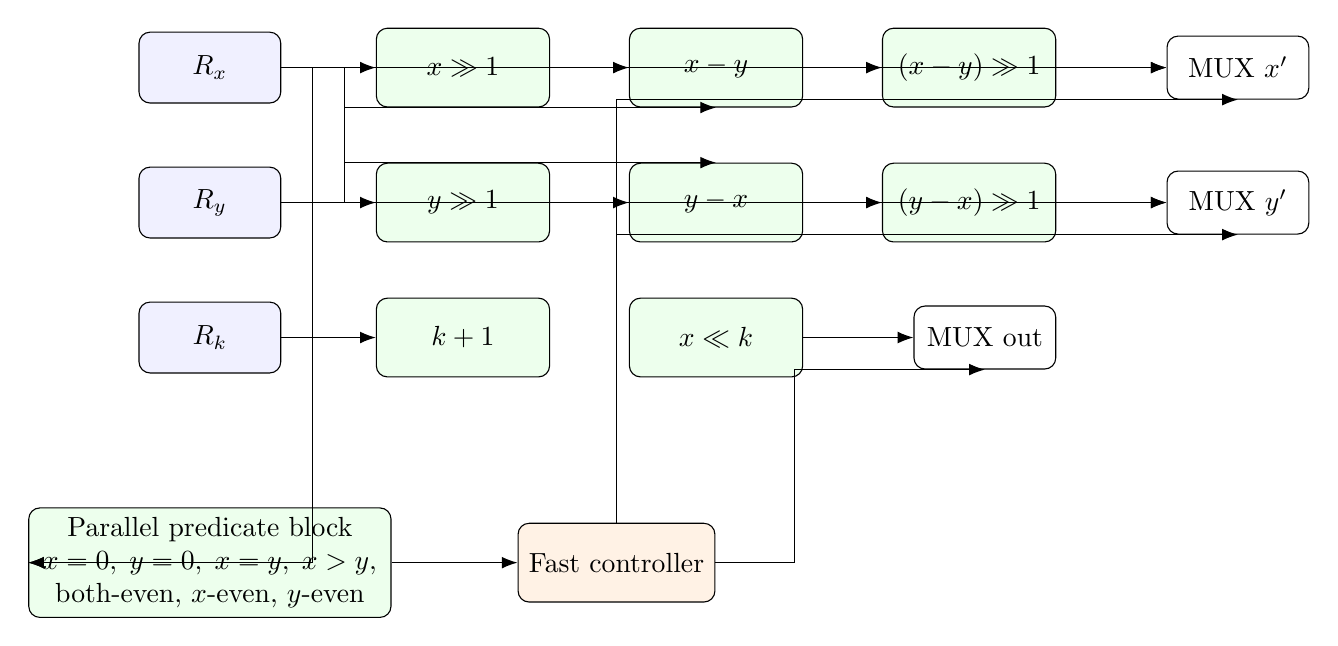
\begin{tikzpicture}[node distance=8mm and 8mm]
  \node[reg] (rx) {$R_x$};
  \node[reg, below=of rx] (ry) {$R_y$};
  \node[reg, below=of ry] (rk) {$R_k$};

  \node[fu, right=12mm of rx] (shx) {$x \gg 1$};
  \node[fu, right=12mm of ry] (shy) {$y \gg 1$};
  \node[fu, right=12mm of rk] (kinc) {$k+1$};

  \node[fu, right=10mm of shx] (subxy) {$x-y$};
  \node[fu, right=10mm of shy] (subyx) {$y-x$};

  \node[fu, right=10mm of subxy] (shsubx) {$(x-y)\gg 1$};
  \node[fu, right=10mm of subyx] (shsuby) {$(y-x)\gg 1$};
  \node[fu, right=10mm of kinc] (gout) {$x \ll k$};

  \node[smallblock, right=14mm of shsubx] (muxx) {MUX $x'$};
  \node[smallblock, right=14mm of shsuby] (muxy) {MUX $y'$};
  \node[smallblock, right=14mm of gout] (muxg) {MUX out};

  \node[fu, below=17mm of rk, minimum width=4.6cm] (cmp) {Parallel predicate block\\$x=0,\; y=0,\; x=y,\; x>y,$\\both-even, $x$-even, $y$-even};
  \node[ctrl, right=16mm of cmp] (ctrl) {Fast controller};

  \draw[->] (rx) -- (shx);
  \draw[->] (ry) -- (shy);
  \draw[->] (rk) -- (kinc);

  \draw[->] (rx) -- (subxy);
  \draw[->] (ry.east) -- ++(8mm,0) |- (subxy.south);
  \draw[->] (ry) -- (subyx);
  \draw[->] (rx.east) -- ++(8mm,0) |- (subyx.north);

  \draw[->] (subxy) -- (shsubx);
  \draw[->] (subyx) -- (shsuby);

  \draw[->] (shx) -- ++(9mm,0) |- (muxx.west);
  \draw[->] (shsubx) -- (muxx);
  \draw[->] (shy) -- ++(9mm,0) |- (muxy.west);
  \draw[->] (shsuby) -- (muxy);
  \draw[->] (gout) -- (muxg);

  \draw[->] (rx.east) -- ++(4mm,0) |- (cmp.west);
  \draw[->] (ry.east) -- ++(4mm,0) |- (cmp.west);
  \draw[->] (cmp) -- (ctrl);
  \draw[->] (ctrl.north) |- (muxx.south);
  \draw[->] (ctrl.north) |- (muxy.south);
  \draw[->] (ctrl.east) -- ++(10mm,0) |- (muxg.south);
\end{tikzpicture}%
}
\caption{Conceptual minimum-latency organization: all candidate branch results are computed in parallel and a controller/multiplexer network commits the correct next values.}
\end{figure}

\subsection*{6.2 Minimum-latency architecture in words}
Because the algorithm has a \textbf{loop-carried dependency}, we cannot eliminate the loop itself. Therefore, ``minimum latency'' means:
\begin{itemize}
  \item \textbf{minimum control steps per iteration}, ideally one cycle per iteration, and
  \item parallel computation of all branch candidates so the next-state decision is only a mux selection.
\end{itemize}

The datapath can therefore update the state in one iteration-cycle as follows:
\begin{itemize}
  \item if both inputs are even, load $x' = x \gg 1$, $y' = y \gg 1$, and $k' = k+1$ simultaneously;
  \item if only one operand is even, shift that operand in the same cycle;
  \item if both are odd, compute both $x-y$ and $y-x$ in parallel and select the correct shifted result using the $x>y$ comparator;
  \item when $x=y$, produce $x \ll k$ immediately through the output shifter.
\end{itemize}

\subsection*{6.3 Functional-unit count}
A natural minimum-latency allocation is:
\begin{center}
\begin{tabular}{lc}
\toprule
Functional unit & Count \\
\midrule
Subtractors & 2 \\
Right shifters & 4 \\
Incrementer & 1 \\
Left shifter & 1 \\
Comparators / parity detectors & parallel status block \\
State/output registers & 4 \\
\bottomrule
\end{tabular}
\end{center}

\noindent
This is not the minimum-area design, but it minimizes execution time by removing most structural conflicts.

\section*{7. Final exam-style answers}
\subsection*{(a) Flowchart}
Use the flowchart in Figure 1. It is based on the standard Stein algorithm with zero checks, equality check, both-even case, single-even cases, and odd-odd subtraction cases.

\subsection*{(b) Data flowgraph}
Use the slide-style sequencing DFG and scheduled DFG in Figures 2 and 3. The controller FSM and its table are given immediately after the DFG, following the same state-graph/table pattern used in the control-unit slides.

\subsection*{(c) ASAP and ALAP scheduling}
With one-cycle arithmetic operations and unlimited resources:
\begin{itemize}
  \item ASAP latency is 2 control steps.
  \item ALAP latency is also 2 control steps.
  \item Zero-mobility nodes are $v_4$, $v_5$, $v_6$, and $v_7$.
\end{itemize}

\subsection*{(d) Minimum-area hardware}
Choose a shared iterative FSMD:
\begin{itemize}
  \item one ALU,
  \item one shifter,
  \item one status/comparator block,
  \item registers for $x$, $y$, $k$, and output,
  \item FSM controller.
\end{itemize}
This minimizes the number of functional units, but increases the number of cycles.

\subsection*{(e) Minimum-latency hardware}
Choose a parallel datapath:
\begin{itemize}
  \item parallel subtractors, shifters, incrementer, and status logic,
  \item branch candidates computed concurrently,
  \item multiplexer-based commit of the correct next-state values.
\end{itemize}
This minimizes the number of cycles per iteration, but increases hardware area.

\section*{8. Conclusion}
The overall HLS reasoning matches the lecture flow:
\[
\text{behavior} \rightarrow \text{CDFG/DFG} \rightarrow \text{scheduling} \rightarrow \text{allocation/binding} \rightarrow \text{FSMD}
\]
which is exactly the sequence emphasized across Slides 5--7.

\end{document}
